\section{Versioned continuation: from nuclei to cell bodies}
\label{sec:continuation}

\subsection{The useful outcome and the missing means}

The beneficiary is a researcher evaluating reproducible offline image measurements. The intended ability is to run an analysis instrument, inspect the objects it predicts, obtain counts and segmentation-derived pixel areas, and determine where it meets a declared reference standard. No laboratory was recruited; these are author-defined research gates, not external laboratory or clinical certification.

The first construction concerns nucleus instances in BBBC039v1. The successor concerns whole-cell instances from the DNA and actin channels of BBBC007v1. Nucleus masks alone do not supply cell-body boundaries. The successor changes the assay, cell line, observation channels, annotation format, and required output. It therefore asks for a different instrument rather than a relabelled first run \citep{bbbc039,bbbc007}.

The initial missing means are deliberately concrete: supported data acquisition, an explicit decoder for reference annotations, an executable analysis recipe, compatible inputs and outputs, independent recomputation of acceptance, and an operating procedure. The recipe operators themselves are established morphology and watershed methods supplied by the authors. Whether that finite grammar contains a qualifying successor is an empirical question; improved ordering cannot manufacture a candidate absent from the grammar.

\begin{practicebox}
\textbf{What a usable first instrument delivers.} A researcher supplies an image within the declared input contract and receives an instance mask, object count, pixel-area records, and inspectable diagnostics. A benchmark qualification supports that contract only. Physical areas require an independently justified pixel scale; a new assay requires its own evidence and acceptance.
\end{practicebox}

\subsection{Frozen data, fields, and acceptance}

The source uses the official BBBC039v1 split: 100 training, 50 validation, and 50 test fields. The 100 training fields supply donor experience and the recipe-selection history; the 50-field validation and test sets assess the emitted source instrument. All 18 test plates also occur in training, so this is not a cross-plate transfer result. The successor uses all 16 complete BBBC007v1 fields: four lexicographically first A9 fields for calibration and twelve remaining fields for test. That structured split is not a random sample of construction tasks. One public successor assay cannot estimate general construction-learning performance.

Both datasets provide public reference annotations and state CC0 terms \citep{bbbc039,bbbc007}. The five compressed archives total 87,775,682 bytes and are identified by hashes in the acquisition and protocol records. Neither a successful download nor a matching hash establishes the scientific adequacy of the labels.

\begin{table}[htbp]
\centering\small
\begin{tabularx}{\linewidth}{@{}P{1.22in}YY@{}}
\toprule
\textbf{Contract} & \textbf{Required quality} & \textbf{Required coverage}\\
\midrule
Nucleus instrument & Mean instance F1 $\geq .70$ under matching with IoU $>0.5$; mean relative count error $\leq .20$; mean foreground Dice $\geq .85$. & Every gate holds separately on the 50 validation and 50 test fields.\\
Whole-cell successor & Mean internal-boundary F1 within 2 pixels $\geq .60$, both over all fields and over reference-boundary-bearing fields; mean count error $\leq .25$; foreground Dice $\geq .80$. & Every gate holds on both four-field calibration and twelve-field test; at least one calibration and two test fields carry reference internal boundaries.\\
\bottomrule
\end{tabularx}
\caption{Acceptance fixed in the registered research comparison. Quality in one column or cohort does not waive another requirement. Area estimates are reported as diagnostics; these gates do not establish biological area accuracy.}
\label{tab:microscopy-contracts}
\end{table}

Instance matching is one-to-one maximum-cardinality matching with IoU strictly greater than $0.5$. Relative count error is $|n_{\rm pred}-n_{\rm ref}|/\max(1,n_{\rm ref})$. The internal-boundary metric uses four-connected inner label boundaries within an eroded foreground, then symmetric precision and recall for boundary pixels within Euclidean distance two. It excludes boundaries adjacent to the background. Reporting a separate mean over fields with true internal boundaries prevents empty-boundary fields from obscuring failure on the actual separation task. Reference regions reconstructed from manual outlines remain conditional on the explicit decoder and border policy in the protocol.

The original BBBC007 boundary-focused setup permits manually outlined nuclei and foreground as inputs, following the work of Jones and colleagues \citep{bbbc007,jones2005}. Our primary contract instead requires both to be constructed from the raw channels; manual inputs appear only in the labelled diagnostic. The collection's historical one-direction boundary percentage and this protocol's symmetric F1 are also different metrics. The reported numbers therefore do not constitute a head-to-head comparison with that historical result.

\subsection{What the constructor can learn in this experiment}

Each classical constructor receives the same 24 supplied recipes, interpreter, target raw channels, four calibration references, and permitted CPU environment. Its adjustable object is the order in which those recipes are evaluated. Greedy coverage of donor performance supplies one revised order; conventional empirical ranking over exactly the same donor table supplies the primary matched comparison. This is an update to a parameter of a supplied finite constructor. It is not discovery of the recipe operators or an autonomous revision of the construction language.

\begin{table}[htbp]
\centering\small
\begin{tabularx}{\linewidth}{@{}P{1.55in}Y@{}}
\toprule
\textbf{Arm} & \textbf{Method and retained means}\\
\midrule
Fixed, no history & A frozen expert-informed order; no donor history or privileged donor recipe.\\
Ordinary reuse & Execute the donor recipe first, then the fixed order without duplicates.\\
Updated, no artifact & Donor-derived greedy-coverage ordering, without privileged donor-artifact execution.\\
Updated with artifact & Execute the donor recipe first, then the greedy order without duplicates.\\
Same-content empirical & Conventional ranking by aggregate donor quality, with the full identical donor table.\\
Full enumeration & Execute all 24 recipes and select with the same calibration quality ordering.\\
\bottomrule
\end{tabularx}
\caption{Six separately executed arms. ``No artifact'' removes privileged donor placement, not the corresponding recipe from the shared bank. The primary contrast is greedy coverage versus same-content empirical ranking.}
\label{tab:six-arms}
\end{table}

Ranked arms stop only at the first candidate satisfying every calibration gate. Each may execute all 24 candidates; a restricted search budget is not used to manufacture an advantage. If none qualifies, the best calibration candidate is retained and labelled unqualified. Full enumeration always evaluates the complete bank. Target scores are not shared across arms. Each selected instrument and its order are sealed before its test stage.

The primary work endpoint is a candidate execution across all four calibration fields. A local advantage requires accepted held-out functionality and a strict reduction in those executions against the same-content empirical arm, without loss of acceptance. CPU time, wall time, checking, donor acquisition, maintenance, and total lineage costs are separate outcomes. Faster prefix search alone cannot establish an overall advantage. The present reproduction uses already exposed data and outcomes; it measures reproducibility rather than producing a new hidden confirmation sample.

\subsection{The practical specialist alternative}

A separately registered CellposeDINO \texttt{cpdino-vitb} route supplies a strong existing specialist. The fixed implementation uses Cellpose 4.2.1.1, pinned DINOv3 source, and a pinned 343,599,997-byte model. It runs on CPU with the frozen inference configuration, without fine-tuning or calibration-based parameter selection. Manual references are excluded from predictor inputs. The upstream documentation identifies this model as the smaller DINOv3-ViT-B member of the CellposeDINO family \citep{cellposeModels}.

The extra pretrained stock is part of the explanation and the cost boundary. Its operation must not be credited to local donor experience or folded into the matched six-arm comparison. Pretraining overlap with the evaluation images is unknown. The code, weights, training-data terms, and DINOv3 terms are distinct rights questions; the recorded scope is research operation, with no established commercial entitlement and no redistribution of upstream source or weights. A working specialist route can be adopted without claiming that it is a newly invented algorithm or an exclusively enabled successor.

\subsection{Preserved failures and representation amendments}

The published preregistration lineage records two failed constructions before target test prediction or scoring. The first encountered Boolean outline storage that violated an integer-only loader assumption. A lossless Boolean-to-integer conversion was registered as a narrow repair. The second encountered RGB raw TIFFs while the observation contract required scalar channels. Its calibration had already exhausted all 24 recipes in every arm, selecting the same unqualified recipe.

The next amendment introduced one common, supplied RGB-to-L convention from Pillow 13, while leaving scalar arrays unchanged. This conversion is generally lossy. It does not recover physical fluorescence or justify a radiometric claim; it changes the represented observation contract explicitly. It applies to raw DNA and actin only, preserves spatial geometry and field membership, and uses the same convention for the classical and specialist routes. The frozen review checked all $2^{24}$ RGB triples against independent fixed-point arithmetic, with a shared Pillow dependency. That is an implementation check, not scientific calibration or external certification.

The specialist preparation also required a narrowly recorded state-loading exception for two nonlearned diameter scalars; trained tensors remained subject to the declared audit. These failures identify integration assumptions, not an opportunity to lower acceptance thresholds. The historical sources and compact review records survive at their published commits. The appendix distinguishes those records from the artifacts produced by the new reproduction and from historical costs that cannot be reconstructed.

\subsection{Results and decision}
\subsubsection{Classical nucleus instrument: the complete source gate fails}

All 24 recipes were evaluated on the 100 donor fields, for 2,400 recipe--field executions. The registered donor selection chose \texttt{r17}. Its training mean count error was 0.591295, so the selected donor was already unqualified on training. The protocol requires continuing the successor comparison even after that failure; it does not permit claiming that an accepted donor enabled an accepted successor.

On the official source cohorts, \texttt{r17} passes every test-set gate but fails the validation count-error gate. Complete source qualification requires both cohorts, so the emitted classical nucleus instrument is \textbf{unqualified}. Its operability and strong performance on some endpoints do not waive the failed requirement.

\begin{table}[htbp]
\centering\small
\begin{tabularx}{\linewidth}{@{}P{1.2in}rrrrY@{}}
\toprule
\textbf{Cohort} & \textbf{Fields} & \textbf{Instance F1} & \textbf{Dice} & \textbf{Count error} & \textbf{Gate verdict}\\
\midrule
Validation & 50 & 0.884357 & 0.910637 & 0.216173 & Fail count error\\
Test & 50 & 0.897397 & 0.931317 & 0.088311 & Pass all three\\
\midrule
Required & & $\geq .70$ & $\geq .85$ & $\leq .20$ & Both cohorts\\
\bottomrule
\end{tabularx}
\caption{Classical source recipe \texttt{r17}. Values are means over fields, rounded to six decimal places; count error is the mean of per-field relative errors, not an error computed from pooled counts. Exact values remain in the machine-readable results.}
\label{tab:classical-source}
\end{table}

\subsubsection{Whole-cell construction: failure and a matched comparison tie}

Every successor arm executed all 24 recipes, or 96 calibration recipe--field evaluations per arm. No candidate met every calibration gate. All six arms selected \texttt{r12} by the same registered fallback ranking and then failed the test boundary requirement. Each of the four calibration and twelve test fields has reference internal boundaries; the all-field and boundary-bearing-field F1 means are therefore equal here. Favorable foreground overlap and count error do not substitute for the missing boundaries.

\begin{table}[htbp]
\centering\small
\begin{tabularx}{\linewidth}{@{}P{1.12in}rrrrY@{}}
\toprule
\textbf{Cohort} & \textbf{Fields} & \textbf{Boundary F1} & \textbf{Dice} & \textbf{Count error} & \textbf{Gate verdict}\\
\midrule
Calibration & 4 & 0.250398 & 0.850357 & 0.086298 & Fail boundary\\
Test & 12 & 0.309897 & 0.861007 & 0.104715 & Fail boundary\\
\midrule
Required & & $\geq .60$ & $\geq .80$ & $\leq .25$ & Both cohorts\\
\bottomrule
\end{tabularx}
\caption{The same selected whole-cell recipe \texttt{r12} and scores in all six classical arms. Each arm separately evaluates its calibration candidates and selected test instrument. All 16 successor fields are boundary-bearing.}
\label{tab:classical-successor}
\end{table}

The primary greedy-coverage versus same-content empirical contrast saves \textbf{zero candidate executions}; both search all 24 and produce the same unqualified selected instrument. There is no local accepted construction advantage and no established lifecycle advantage. This is an observed tie in selected instrument, quality, and candidate count on this comparison. Runtime measurements can differ; the result is not a statistical equivalence claim over a population of construction tasks.

The full-enumeration control also exhausts the bank and fails. Thus the result is not caused by denying a conventional method sufficient search. Under these fixed operators, observations, calibration fields, and gates, another ordering alone cannot produce an accepted candidate. This conclusion applies to the tested bank, not to all methods for cell segmentation.

\paragraph{A controlled explanation of convergence.}
The six arms are deterministic policies over one supplied grammar, not six separately prompted language models. Their original executions contain four distinct proposed orders. All 96 recipe--calibration-field records per arm agree in prediction hashes and scientific metrics when aligned by recipe and field. A separately frozen diagnostic called the unchanged constructor with 33 order/settings interventions, comprising 30 unique orders. It replaced only the expensive evaluator boundary with an explicitly labelled adapter returning the retained calibration scores. Every replay exhausted 24 candidates and selected \texttt{r12}; there were 792 cached evaluator calls and no new image inference in this part. The highest calibration boundary F1 in the whole bank was 0.250398. The observed convergence is explained by shared candidate failure and the common fallback ranking, not identical ordering or independent model agreement. This is a mechanism check on exposed records, not a fresh task or evidence of improved construction learning.

\subsubsection{Diagnostics: what the failure does and does not localize}

The unchanged donor artifact, applied as a labelled diagnostic on the twelve successor test fields, obtains boundary F1 0.072995 and foreground Dice 0.537565 and is unqualified. The separate oracle-input diagnostic supplies manual nuclei and manual foreground to \texttt{r12}; its test boundary F1 is 0.671256, Dice 0.999933, and count error 0.159935. It meets the numerical test gates only with privileged reference-derived inputs, so it is \textbf{not a qualified raw-channel instrument} and not a primary arm.

The diagnostic supports investigating how reliable seed nuclei and foreground can be constructed from permitted observations. Because both inputs change together, it does not isolate which one is decisive, demonstrate a practical way to obtain them, or establish success on a new cohort. A new boundary method is one possible next construction; better construction of its input means is another. The reference-assisted result must not be presented as an ordinary deployment option.

\paragraph{Separating the two input interventions.}
A new diagnostic froze \texttt{r12}, the unchanged acceptance criteria and the four already exposed calibration fields before executing a $2\times2$ component comparison. No target test pixels were decoded. Each condition called the existing segmentation code and was scored by both the producer's metric code and the separately implemented checker. The baseline matched all archived calibration prediction hashes and scores. The combined intervention matched a new call to the unchanged producer's oracle path on these same four fields; no prior combined-reference calibration output was claimed.

\begin{table}[htbp]
\centering\small
\begin{tabularx}{\linewidth}{@{}YrrrP{.78in}@{}}
\toprule
\textbf{Calibration inputs} & \textbf{Boundary F1} & \textbf{Dice} & \textbf{Count error} & \textbf{Numerical gate}\\
\midrule
Raw seeds, raw foreground & 0.250398 & 0.850357 & 0.086298 & Fail\\
Reference seeds, raw foreground & 0.195353 & 0.829797 & 0.111399 & Fail\\
Raw seeds, reference foreground & 0.615828 & 0.999903 & 0.090194 & Pass\\
Reference seeds and foreground & 0.714909 & 0.999903 & 0.165064 & Pass\\
\bottomrule
\end{tabularx}
\caption{Fixed-recipe interventions on four exposed calibration fields. A numerical pass with reference foreground does not qualify a raw-input instrument or imply that every individual field passes. All sixteen component masks received separate-code rescoring; eight additional producer-control segmentations were charged.}
\label{tab:component-diagnostic}
\end{table}

Foreground replacement alone increased mean boundary F1 by 0.365430, whereas seed replacement alone decreased it by 0.055045. This favors investigating foreground recovery before a seeds-only repair in this implementation. The raw-foreground branch unions its mask with the supplied seeds, so changing seeds can also affect foreground; these are software-branch interventions, not isolated biological causal effects. Nearly perfect Dice with reference foreground is expected from the privileged input. The complete registration, code, masks, controls and replay checks are in \texttt{construction/diagnostics/}. Neither diagnostic supplies untouched confirmation cases or changes the original failure verdicts.

\paragraph{Constructing and rejecting one practical repair.}
The diagnostic led to one separately frozen, assistant-authored ordinary composition: take the union of the pinned specialist's final whole-cell instances as a foreground proposal, then apply the unchanged \texttt{r12} DNA-seeded watershed. The actual composition was executed on the four saved specialist calibration predictions, whose original raw-input inference and identities are retained. No reference foreground or nuclei were supplied to this candidate. Its mean boundary F1 was 0.296809, Dice 0.861057, and count error 0.081112. It improved the classical boundary endpoint but remained below the fixed specialist's 0.386561 and failed the unchanged 0.60 criterion.

The frozen stop rule was enforced: zero target test fields were scored, no parameter was tuned, and no new neural inference was performed for this failed candidate. The reusable raw-input command is included, but full fresh execution of that command is not claimed. The observed result is a failed composition from identified, previously executed constituent outputs. Its 3.263 CPU seconds and 1.755 wall seconds are additional work. The original four specialist fields already incurred 122.037 CPU seconds in segmentation (122.637 CPU and 122.650 wall seconds at the enclosing field boundary); these constituent costs are attributed, not charged a second time. The registration, implementation, masks, adverse outcome and stop receipt are in \texttt{construction/repair/}. Reliable foreground remains an unmet requirement; this available substitution did not construct it.

\subsubsection{Pretrained specialist: a qualified first route, a failed successor}

The fixed CellposeDINO route meets every nucleus gate on both official 50-field cohorts. Its test instance F1 is 0.949103, foreground Dice 0.967232, and mean relative count error 0.070837. It is therefore \textbf{qualified for the declared source research contract}. The practical construction consists of integrating and operating the pinned existing specialist with the input adapter, reference interpretation, measurements, and checks. It does not establish that the local constructor learned the specialist's competence or that pixel-area estimates are validated biological measurements.

The same specialist fails the whole-cell boundary gate on both calibration and test. Its test boundary F1 is 0.505568, below the required 0.60, despite passing the foreground and count gates. All 16 successor fields carry reference internal boundaries, so the boundary-bearing-field mean also fails. The successor is \textbf{unqualified}.

\begin{table}[htbp]
\centering\small
\begin{tabularx}{\linewidth}{@{}P{1.52in}rrrrY@{}}
\toprule
\textbf{Cohort} & \textbf{Fields} & \textbf{Primary F1} & \textbf{Dice} & \textbf{Count error} & \textbf{Gate verdict}\\
\midrule
Nuclei: validation & 50 & 0.953878 & 0.967388 & 0.066573 & Pass all three\\
Nuclei: test & 50 & 0.949103 & 0.967232 & 0.070837 & Pass all three\\
Cells: calibration & 4 & 0.386561 & 0.860566 & 0.130928 & Fail boundary\\
Cells: test & 12 & 0.505568 & 0.886682 & 0.200904 & Fail boundary\\
\bottomrule
\end{tabularx}
\caption{The fixed pretrained specialist on all 116 registered fields. Primary F1 means instance F1 for nuclei and internal-boundary F1 for cells; the different gates are given in Table~\ref{tab:microscopy-contracts}. Entries are field means rounded to six decimals. The source qualifies only because both nucleus cohorts pass; the successor requires both whole-cell cohorts and fails.}
\label{tab:specialist-results}
\end{table}

On this successor test cohort, the specialist achieves higher boundary F1 than the selected classical recipe, but also has higher count error; neither meets the complete contract. Its additional pretrained stock is a distinct resource, not the product of the local ordering update. The specialist was chosen after classical source outcomes and registered before its own inference. Potential pretraining overlap with these public images is unknown. These are findings from an exposed reproduction, not evidence of unseen-data generalization or a newly concealed comparison. Figure~\ref{fig:microscopy-examples} shows two fields chosen by declared test order, without using their scores; the complete cohorts determine the verdicts.

\subsubsection{Measured work and its boundary}

The completed classical run records 696.935 CPU seconds and 696.703 wall seconds across donor construction, source evaluation, and successor construction/evaluation, including the two labelled diagnostics. The separate completed 116-field specialist session records 4,969.507 CPU seconds and 4,970.035 wall seconds. These are measured stage or session boundaries from this reproduction. They exclude dependency setup, data acquisition, independent verification, authoring, upstream pretraining, unavailable earlier execution costs, and economic costs. They are not a whole-lineage total or a monetary price. The full report retains per-arm times alongside candidate counts so an endpoint tie is not misrepresented as identical timing.

The classical ledger records three completed attempts and no interrupted or orphaned attempt. Its negative interruption flag describes that recorded state, not verified absence of unrecorded work. The origin of 138 byte-identical residual files remains unresolved: they could be copies or products of additional execution. Any associated extra work and cost are therefore unknown. The projection preserves the measured charges and does not establish that all classical execution or cost has been captured.

The new order/component diagnostic adds 8.465 CPU seconds and 7.058 wall seconds, including its 24 actual segmentations and separate-code scoring; the order interventions themselves use cached scores. Its reproduction adds a separately recorded 8.896 CPU seconds and 7.278 wall seconds. These costs are outside the original classical stage total. The qualification packet separately preserves the installer failure, repair tests and real candidate-package inference. Nested operation and wrapper timings must not be counted twice; total authoring, human effort and monetary billing remain unknown.


\subsection{What the continuation can establish}

A qualifying first instrument establishes a bounded computational capability on the recorded data and input contract. A successor failure localizes a remaining requirement; it must remain a failure even when foreground or count diagnostics look favorable. A tie against same-content empirical ranking supplies no evidence of a better constructor. Failure to qualify from a finite recipe bank does not prove that no segmentation method can qualify.

The observed classical failure directs the next experiment toward the means of producing adequate boundaries, including reliable seed nuclei and foreground. The rational next experiment therefore follows the diagnosed missing means. If the bank is exhausted, another ordering of the same bank has no acceptance gain to discover. A boundary-specific representation, observation, algorithm, or licensed specialist is a candidate next construction. It must be frozen and compared on a new confirmation cohort, with strong complete alternatives and the costs of acquiring that capability. The current result motivates that question; it does not answer it by proposing the remedy.


\begin{figure}[htbp]
\centering
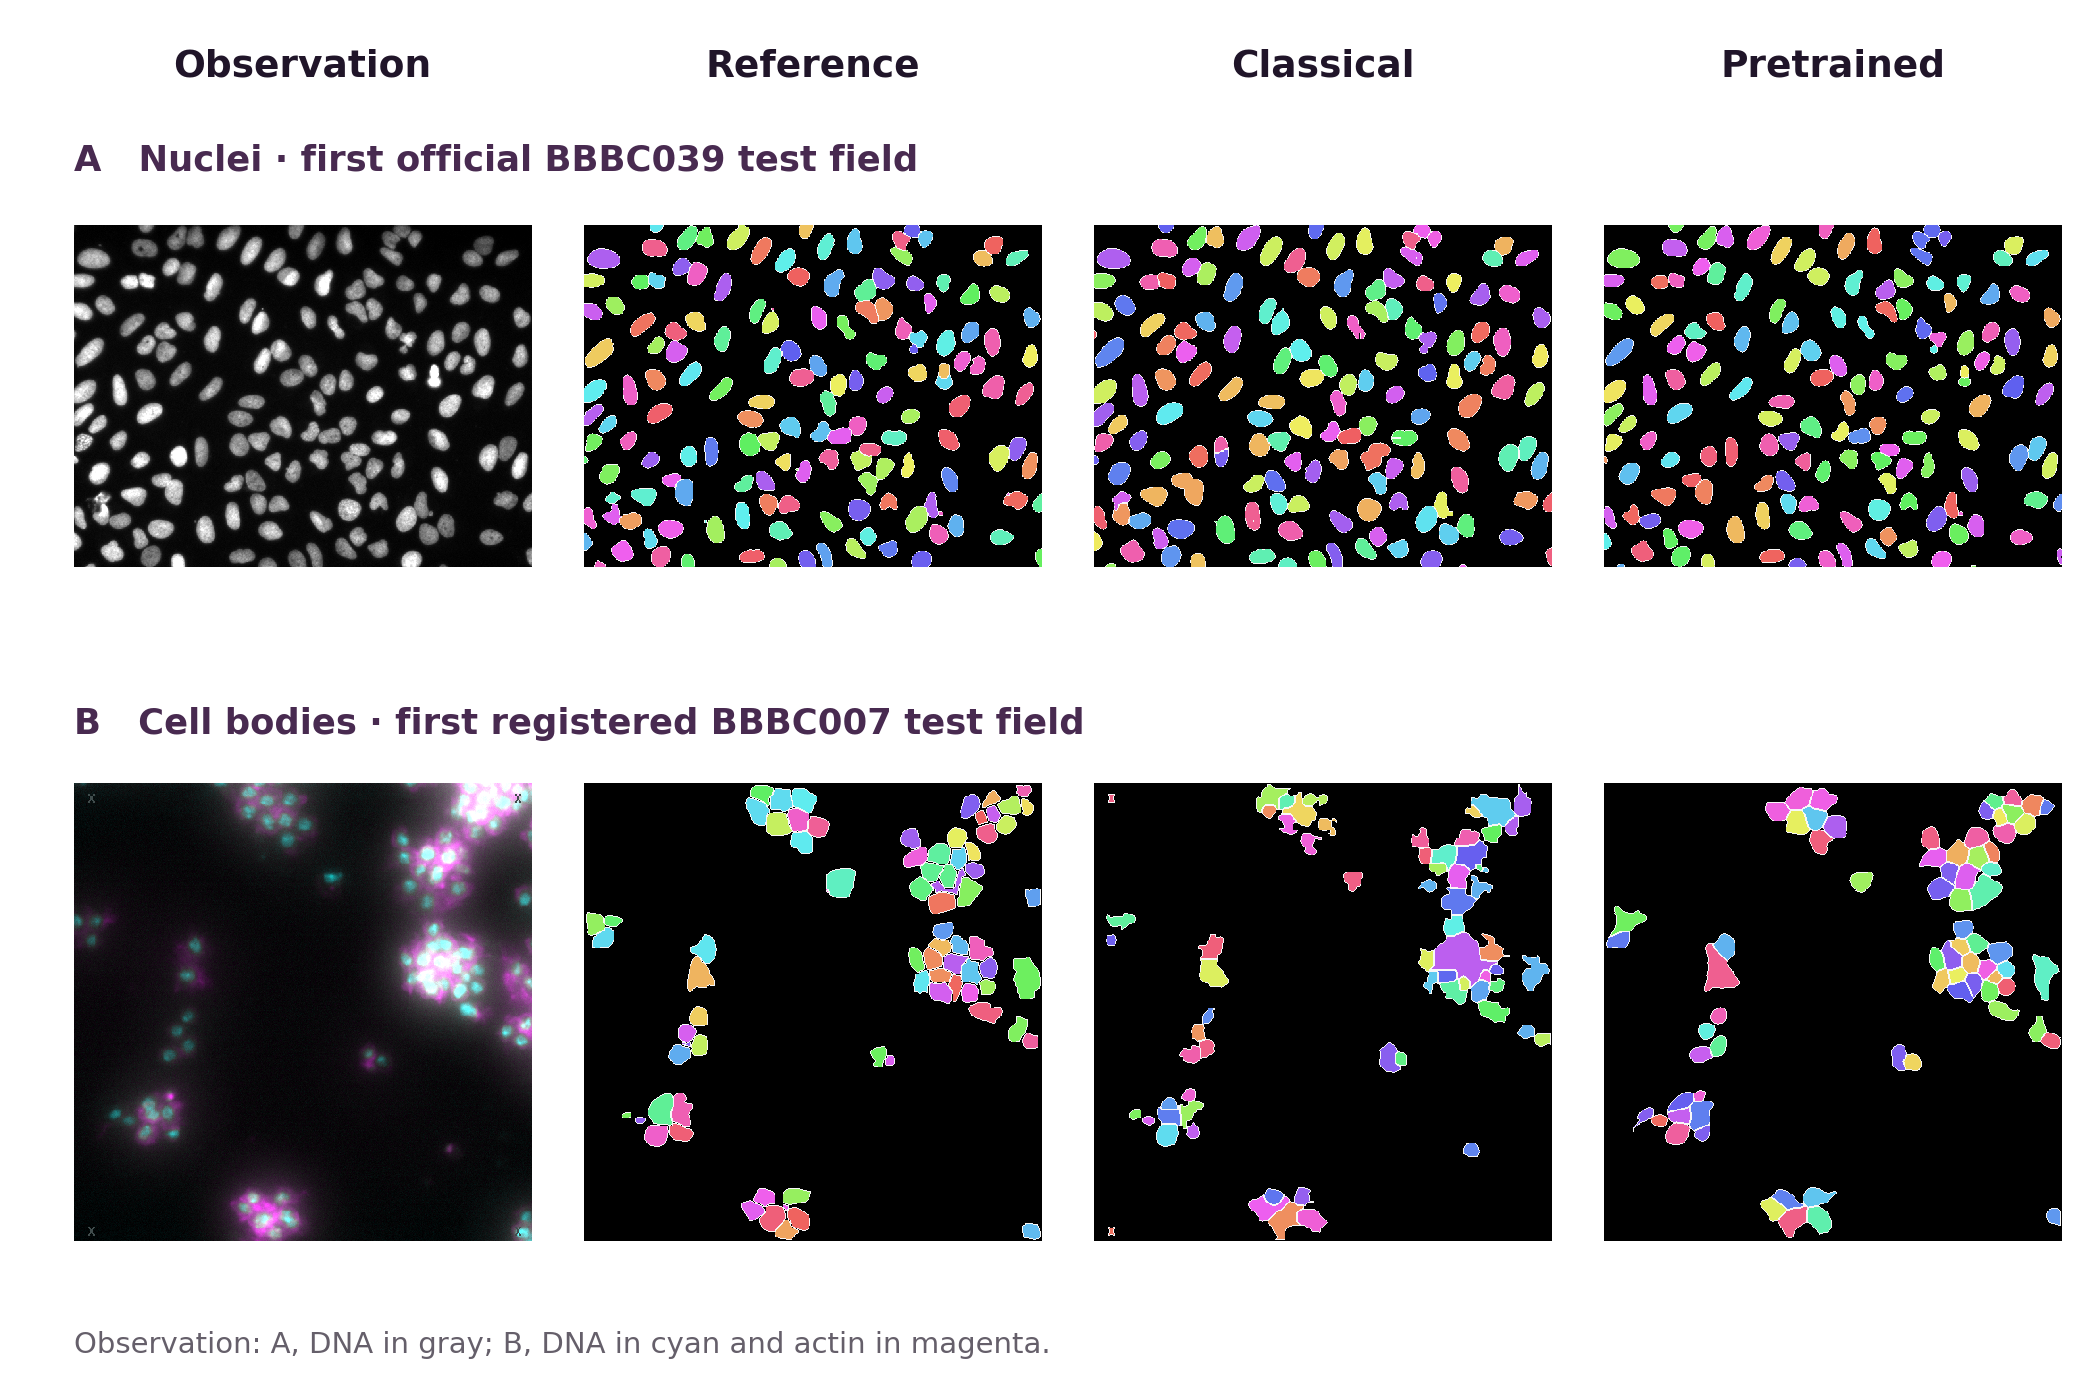
\includegraphics[width=\linewidth]{construction/figures/protocol-first-fields.png}
\caption{Two test fields selected by declared order, without using their scores: the first official BBBC039 test field and the first registered BBBC007 test field. Columns show the canonical observation, registered decoded reference, classical prediction (\texttt{r17} for nuclei; \texttt{r12} for cells), and fixed pretrained prediction. Full fields are shown without cropping. Each observation channel uses linear clipping at its first and ninety-ninth percentiles \emph{for display only}; inference and scoring inputs are unchanged. Colors distinguish instances within a panel and do not imply correspondence across panels. White inner edges aid visibility. The BBBC007 masks retain the registered complete-in-frame convention. These examples illustrate outputs; they do not replace the cohort results. Exact field identities, input and mask hashes, display ranges, and rendering source are retained in the accompanying figure receipt.}
\label{fig:microscopy-examples}
\end{figure}
\FloatBarrier
